\documentclass{article}


\usepackage{arxiv}

\usepackage[utf8]{inputenc} % allow utf-8 input
\usepackage[T1]{fontenc}    % use 8-bit T1 fonts
\usepackage{hyperref}       % hyperlinks
\usepackage{url}            % simple URL typesetting
\usepackage{booktabs}       % professional-quality tables
\usepackage{amsfonts}       % blackboard math symbols
\usepackage{nicefrac}       % compact symbols for 1/2, etc.
\usepackage{microtype}      % microtypography
\usepackage{lipsum}		% Can be removed after putting your text content
\usepackage{subfigure}

\usepackage[toc,page]{appendix}
\usepackage{amsmath}
\usepackage[ruled ]{algorithm2e}
\usepackage{tikz}
\usetikzlibrary{fit,positioning,arrows,automata,calc}
\tikzset{
	main/.style={circle, minimum size = 5mm, thick, draw =black!80, node distance = 15mm},
	invis/.style={circle, minimum size = 10mm, thick,  node distance = 15mm},
	connect/.style={-latex, thick},
	box/.style={rectangle, draw=black!100}
}


\title{Bachelor Project Report: \\ Multiple Object Tracking with Point Patterns}

%\date{September 9, 1985}	% Here you can change the date presented in the paper title
%\date{} 					% Or removing it

\author{
  Simon Giebenhain\thanks{The work was done as a Bachelors Project supervised by Prof. Bastian Goldlücke. My code and videos displaying my tracking results can be accessed via \href{https://github.com/SimonGiebenhain/tracking}{GitHub}} \\
  Department of Computer Science\\
  University of Konstanz\\
  \texttt{simon.giebenhain@uni-konstanz.de} \\
}

\begin{document}
\maketitle

\begin{abstract}
Multiple Object Tracking (MOT) has been a subject of research for many years. This paper introduces a new kind of MOT problem, working on unlabeled point detections made of each objects unique point pattern. Next to position, also the orientation of objects becomes of interest. The problem was inspired by trying to track birds based on three-dimensional detections of markers on the their backs. Having access to occlusion free three-dimensional detections makes assigning detections to objects easy. Therefore this task is handled with a simple MOT framework, which can be used with any Single Object Tracker (SOT). A Kalman Filter (KF) based SOT with a few additions tailored for the specific MOT problem is introduced. Experiments show that these additions to the regular KF greatly improve MOT performance. Additionally a neural network based approach is described, which performs worse than the KF approach, but shows promising noise resistance.
\end{abstract}


% keywords can be removed
%\keywords{First keyword \and Second keyword \and More}


\section{Introduction}
%IDEA why use patterns for MOT etc.
Multiple Object Tracking(MOT) refers to the task of identifying and maintaining some desired properties of objects of interest over time.
This paper introduces two Multiple Object Tracking methods which work on unlabeled point detections. Each object is equipped with a point pattern consisting of multiple single markers. The markers are what is being detected. In this paper the desired properties are location and orientation. The work is tailored towards MOT of birds in three-dimensional space, with patterns being defined by the position of four markers. A more precise formulation of the problem is given in section \ref{problem_def}.
\begin{figure}[!htbp]
	\begin{center}
		\subfigure[Flying birds]{%
			\includegraphics[scale=0.26]{img/overview_data.png}
		}
		\subfigure[Detailed top-down-view]{%
			\includegraphics[scale=0.27]{img/detailed_data.png}
		} 
		
	\end{center}
	\caption{\textbf{Detections and tracking results} - Gray stars represent detections. Colorful circles show the points where markers of tracked birds are expected, based on tracked position and orientation. The lines show past movement of birds. (a) Shows some birds flying towards the ground, while others are stationary. (b) Gives a detailed view of four birds. One can see a false positive detection next to the dark blue bird. Lots of detections are missing, e.g. only one of the four markers of the red bird are currently visible.}
	\label{data_impression}
\end{figure} \\
Usually MOT is performed on video data as the most common use-cases are sports tracking, tracking of pedestrians and in autonomous driving. While this paper technically deals with MOT, this setting is quite different, since precise three-dimensional point detections instead of videos are used, alleviating occlusion problems. Together with a frame rate of 30 frames per second the detection-to-track-assignment, which is the main challenge of the classical MOT problem, becomes easy. The difficulty shifts towards accurate Single Object Tracking (SOT), especially the precise tracking of orientation remains challenging. 
%TODO was noch? 
\\
Therefore, I propose two approaches for SOT, which can be embedded in a simple MOT-framework to track multiple objects at once. This framework is described in section \ref{approaches}. \\
Section \ref{kf_appraoch} introduces the first SOT approach, which is based on a Kalman Filter (KF). The fundamental difficulty of this SOT approach is to estimate the assignment of the detections to the markers, as knowing these correspondences is necessary for the KF to work.
\\
Section \ref{dl_approach} introduces a recurrent neural network based approach for SOT. I formulate a general architecture, in which an embedding neural network transforms the input of each time step and feeds it into an Long-Short-Term-Memory  network (LSTM). Multiple possible encoder architectures are considered, as this is the most crucial part of the network. The detections at each time step are point clouds of varying number of points, and therefore the encoder has to be permutation invariant as well as resistant to noise, missing detections and false positive detections.\\
I validate my design choices for both approaches by running experiments on data with varying degrees of noise, missing detections and false positive detections. In order to conduct these experiments, I had to generate data with known ground truth. The data generation process is described in section \ref{results}. A quantitative comparison of both approaches and a short discussion is given in section \ref{comparison}. The experiments showed that the KF approach currently achieves superior tracking performance and is more flexible than the neural network, as new data could require retraining the complete neural network. %TODO: noch mehr zusammenfassung anstatt nur Gliederung aufzulisten
\\
Multiple ideas for improving both methods are presented in section \ref{future_work}. %TODO: more? das vielleicht sogar weg?


%TODO: am ende noch kleine conclusion, wie zB. aktuell KF besser aber NN zeigt potential

% TODO experiements show that simple KF in simple MOT framework is capable of doing MOT, which supports focussing on SOT




\subsection{Data Capturing Setup}
\label{data_setup}
% markers humanly designed, room for improvement

%TODO this gives some context

%TODO marker setup 
This section explains how the data is being captured. Images of the data are shown in figure \ref{data_impression}.
The data was captured inside of a large room with a 2D array of infrared cameras filming downwards from above. Due to a multitude of cameras the detections are precise in three-dimensional space and occlusion does not occur. Each bird is equipped with a tiny backpack which has space for 4 infrared reflecting markers, positioned in a unique pattern. There can be small elevations on the backpack, meaning that the specified pattern can be three-dimensional instead of just lying in one plane. Using these patterns enables to predict the orientation and position of the birds in three-dimensional space. All individual markers are the same, meaning that it is impossible to distinguish between single detections.  Although the room was painted such that a minimal amount of infrared light gets reflected from anything else than the infrared markers, there is still a substantial amount of false positive detections. Similarly markers are often not detected by the cameras. These kinds of noise pose the main problem to be addressed in this paper.   %These patterns are specified by hand by the supervisers of the experiment. An analysis of the performance of different patterns could lead to insights which allow for the design of better patterns. However such proceedings are out of scope for this work and may be subject to future research if need be.

%The aforementioned infrared cameras feed information directly to the VICON Tracker3 system, which puts all detections into a unified three-dimensional coordinate system. The input to the tracking algorithms presented here is therefore a set of unlabelled 3d detections for each time frame. The VICON system produces detections accurate to the millimeter. Therefore this work assumes that there is little noise in the true positive(TPs) detections.






\section{Related Work}
\label{related_work}
% research focuses on pedestrians,  and visual similarity, pose is uncommon, solely position no rotation
% check tracking the trackers and summarize some common approaches

Most of the MOT research focuses on tracking pedestrians or vehicles, as surveillance and autonomous vehicles are two driving industry applications for MOT. These approaches usually apply a tracking-by-detection paradigm, where an object detector locates objects of interest in each frame and the MOT algorithm associates these detections to the maintained tracks. This procedure is called detection-to-track-assignment. This way the algorithm can focus on the information nearby the detected objects and discard seemingly irrelevant information. The detection-to-track-assignment is the most crucial point of these approaches and commonly performed with visual features drawn from the detected bounding boxes. \cite{tracking_the_trackers} found  that the most defining feature of the best performing models on the MOT15 benchmark (\cite{MOT15}) and MOT16 benchmark (\cite{MOT16}) is a good affinity measure using appearance features.


\cite{milan_rnn_tracking} present a very general, recurrent neural network based model for MOT, which is trained end-to-end and does not use any information besides the location. They argue that applying deep learning to MOT is far from trivial. In MOT the tracked states are continuous, whereas the detection-to-track-assignment is a discrete assignment problem. The number of tracked objects is arbitrary and death and birth of tracks have to be handled. These circumstances make it hard to design a architecture which can handle this variety of data. Their results reflects this reasoning, as the version of their model which uses an LSTM architecture for the detection-to-track-assignment performs slightly worse than the version using the Hungarian Algorithm (HA) for the detection-to-track-assignment. For this reason I choose to use the HA.

The work of \cite{3d_kalman}  uses a regular KF for tracking objects in three-dimensional space, where the state is composed of position, velocity, heading angle, and lengths describing the size of the bounding box of an object. They achieve state-of-the-art-results on the 3d MOT challenge on the KITTI dataset (\cite{kitti}), while being the fastest method with a large margin among the top algorithms. Their input are the detected bounding boxes from \cite{PointRCNN}, which achieves the state-of-the-art results on the the 3d object detection challenge from the KITTI dataset, despite only using LiDAR point clouds and no RGB images at all. Using these state-of-the-art detections might explain their superiority in the 3d MOT challenge. Their work supports the choice of following a KF approach to tackle the problem at hand.

\paragraph{Differences to regular MOT} The MOT variant discussed in this paper naturally follows a tracking-by-detection scheme, as 3d detections are the only available source of information. However the task at hand differs substantially from the regular MOT setting. When tracking pedestrians the scenes are usually very crowded and troubled by occlusion. Then an affinity model relying on visual appearance is crucial. The point detections in this work have high precision and are three-dimensional, which resolves occlusion problems. Therefore the detection-to-track-assignment is relatively easy most of the time and the MOT problem can be tackled by multiple SOTs and the HA for assigning the detections to the tracks.\\
 However even a perfect detection-to-track-assignment does not guarantee a good tracking performance, as multiple detections are assigned to each object, without knowing which detection corresponds to which marker of the pattern. In order to estimate the position and orientation correctly, an exact detection-to-marker-assignment is required.\\
The task is complicated further by frequent missing detections and detections, which do not correspond to one of the markers, so called false positive detections. Missing detections especially become a problem when less than two detections are present for multiple frames, as no unique orientation can be determined. Not identifying a false positive detection as such, can potentially disrupt the orientation estimation. Therefore the applied SOT method has to be  robust against such noise. Additionally, a strong motion model and using temporal information effectively seem to be crucial. \\


\section{Problem Formulation and Notation}
\label{problem_def}

This section introduces the notation used throughout the rest of the paper while stating the problem mathematically. The task is to estimate the position and orientation at every time step for every object, based on a sequence of noisy detections of the unique point patterns over time. \\

In this formulation the patterns of the occurring birds have to be known beforehand. Let $N$ be the number of known patterns, and let $N_t$ be the number of present objects in frame $t$.\\
Each pattern is made up out of $K$ markers. A pattern defines the arrangement of the $K$ markers, which are $d\text{-dimensional}$ points, in space. The pattern of the $n\text{-th}$ object is denoted by $$m^{(n)} = 
\begin{pmatrix}
m^{(n)}_1 \\
\vdots \\
m^{(n)}_K
\end{pmatrix} \in \mathbb{R}^{Kxd}, \text{ where the } k\text{-th} \text{ row holds the } k\text{-th} \text{ marker }, m^{(n)}_k \in \mathbb{R}^d$$

Let $T$ be the number of total time steps, then the input is a sequence of detected point clouds denoted by $\smash{\left( \mathcal{X}^{(t)} \right)_{t=1}^T}$, where $\smash{\mathcal{X}^{(t)} \subset \mathbb{R}^d}$. 
It is important to note here that $\smash{\mathcal{X}^{(t)}}$ is a set of $d\text{-dimensional}$ points, meaning that we have no prior information which detection belongs to which marker of which object. While $\smash{\mathcal{X}^{(t)}}$ conceptually is a set, the detections are stored in such a way that there is an arbitrary ordering to them. I will reference the corresponding but ordered detections with $\smash{X^{(t)}}$. \\

For each object the values to estimate are the 
$$ \text{positions } \left(p^{(t)}_1\right)_{t=1}^T, \dots,\left(p^{(t)}_N\right)_{t=1}^T \text{ and rotations } \left(r^{(t)}_1\right)_{t=1}^T, \dots,\left(r^{(t)}_N\right)_{t=1}^T$$ 
%TODO: where to put thi, maybe related work (https://pdfs.semanticscholar.org/b12a/a54a6676f2e2614c8d463334799d6cfdb93e.pdf says the other way around and http://read.pudn.com/downloads182/ebook/848457/Wiley.Global.Positioning.Systems.Inertial.Navigation.and.Integration.2nd.Edition.Jan.2007.pdf)
For $d=3$ there are many common way to represent rotations. Next to the canonical representation as a rotation matrix, there are for example Euler angles and quaternions. Euler angles are a minimal representation since it only requires 3 parameters. However, they exhibit singularities, which correspond to a gimbal lock configuration, where large changes in the Euler angles are required to represent small changes in the actual rotation, \cite{manifolds}. Therefore, Euler angles are generally considered inferior to quaternions in controlling and tracking tasks. 

The task is to come up with the $$ \text{ position estimates } \left(\hat{p}^{(t)}_1\right)_{t=1}^T, \dots,\left(\hat{p}^{(t)}_N\right)_{t=1}^T \text{ and rotation estimates } \left(\hat{r}^{(t)}_1\right)_{t=1}^T, \dots,\left(\hat{r}^{(t)}_N\right)_{t=1}^T$$ which minimize some desired error. The Multiple Object Tracking Accuracy (MOTA) and Multiple Object Tracking Precision (MOTP) metrics introduced in \cite{mot_metrics} could be of interest. The MOTP metric has to be adapted in order to account for the whole patterns:

\begin{equation}
	\text{Pose-MOTP} := \frac{1}{T\cdot \sum_{t=1}^TN_t \cdot K}\sum_{t=1}^{T}\sum_{n=1}^{N_t} \sum_{k=1}^{K} \left\| \text{Rot}(r^{(t)}_n)m^{(n)}_k + p^{(t)}_n - \text{Rot}(\hat{r}^{(t)}_n)m^{(n)}_k + \hat{p}^{(t)}_n \right\|_2
\end{equation}

Here the function $\text{Rot}(r)$ maps the rotation representation $r$ to a rotation matrix. Note that the MOTP metric disregards missed tracks, false positive tracks and ID-switches. These details are skipped in the formula above for simplicity reasons.

I constrain the problem to the specificities of the bird data by fixing the dimensionality $d=3$ and the number of markers per pattern $K=4$. Having $d=3$ also seems to be the most applicable case in general.


\section{My Approaches}
\label{approaches}
I followed two major approaches to solve the specific MOT problem described above, a KF approach and a modern deep learning approach. Both approaches are embedded in the same MOT framework, a tracking-by-detection framework which uses multiple SOTs combined with some simple heuristics to mange multiple tracks. The framework is depicted in figure \ref{flow_chart}. In the following I describe the components of this framework in more detail.


%TODO notation in diagramm anpassen!
\begin{figure}[!htbp]
	\begin{center}
		\includegraphics[scale=0.2]{img/MOT_framework.png}
		\caption{ \textbf{MOT Framework} - 
			(1) Each SOT predicts location and rotation for frame $t$. (2) \& (3) The detections of frame $t$ are associated with the predicted positions using the HA with the possibility for non-assignments (4) The SOT get the assigned detections as input to correct their internal state and make a more accurate estimation for the current position and rotation. These estimates are stored. (5) \& (6) The track management unit gets informed which tracks where unassigned and decides whether to discontinue the track or not. (7) \& (8) The track management unit gets all unassigned detections. If it detects the pattern of a untracked bird, a new track is initialized. }
		\label{flow_chart}
	\end{center}
\end{figure}

\paragraph{Single Object Tracker} 
For each present object there is a SOT, which makes predictions for the position and orientation of the object in the next frame. These predictions are used by the \emph{data association unit} to assign the detections to the objects. The SOTr then gets its assigned detections as input, in order to make a more accurate estimation for the position and rotation for the current frame and to correct its internal state.\\
This unit is formulated generic, such that multiple methods can be used as SOT. Section \ref{kf_appraoch} describes a KF based SOT and section \ref{dl_approach} describes a neural network based approach.

\paragraph{Data Association or Detection-to-Track-Assignment Unit} 
Due to the fact that the tracking takes place in three-dimensional space, the detection-to-track-assignment is relatively simple, as  empirical results suggest (see Section \ref{results}). Therefore this work is limited to a simple data association scheme based on the HA. Additionally to the standard HA there is a fixed cost for not assigning a detection to one of the $K$ markers of an object and for leaving one of the $K$ markers of an object unassigned.


\paragraph{Track Management Unit} This unit handles the task of creating new tracks and deleting tracks which have been lost. The latter task is done in the simplest way possible. Tracks are deleted, if they were not assigned any detection for more than fixed number of frames.\\ 
The creation of new tracks has to be done carefully in order to prevent ID-switches. Therefore, a new track is only initialized when a pattern of one of the objects, which are not currently tracked, exactly matches a subset of the unassigned detections. For larger $K$ it would be sufficient if a subset of the pattern matches a subset of the detections almost perfectly. However since $K=4$ for the bird data this would lead to falsely creating new tracks frequently.\\
In this case the algorithm deciding whether new tracks are created can be described as follows: All unassigned detections are clustered using an agglomerative, hierarchical clustering scheme with the euclidean distance as a metric. Clusters are formed by cutting the dendrogram where links have larger distances than the largest distance between points in a pattern. all clusters with 4 or more points are considered as candidates. Then a pattern matching algorithm developed in \cite{umeyama} is iteratively applied to the cluster paired with one of the patterns of an untracked object. The pattern matching algorithm finds the similarity transformation (rotation, translation and scaling), that minimizes the mean squared error between the transformed detections and the pattern. For this method to work, the correspondences between detected points and points of the pattern have to be known. This assignment is estimated with a similar method as described in section \ref{dtma}, just without any prior knowledge of the position and orientation. After ordering the detections correctly the pattern matching algorithm can be applied. If the returned mean squared error is below a certain threshold, the pattern is considered a match and a new track is initialized with the calculated position and orientation. The threshold is chosen very low, such that new tracks are only initialized with very high confidence.

 


\subsection{Kalman Filter Approach}
\label{kf_appraoch}
This section describes a SOT, based on a KF approach, which can be used in the MOT framework described above. The KF is a well known method across many different fields and is frequently applied to tracking problems and constitutes an interesting baseline to the MOT problem specified above. The KFr is an algorithm that aims at uncovering the underlying state of a system, given only a sequence of noisy measurements originating from the system. A description of the system and measurements in a probabilistic settings gives rise to a graphical model depicted in figure \ref{graphical_model}. The KF follows a predict-correct mechanism. It predicts the state for the next time step as a probability distribution. Once a new measurement is available the probability distribution estimating the state is corrected with the new information. If the reader is not familiar with the KF and its variants, I refer the reader to \cite[Chapter~19]{prince}.

If the underlying system is a Linear Dynamic System (LDS), only only Gaussian noise is present and the dynamics and noise parameters are known the KF can be proven to be the optimal estimator for the system state with respect to the mean squared error. \\
The system at hand is not linear, due to the inherent non-linearity of rotations. For non-linear dynamic systems there are extensions of the KF, such as the Extended Kalman Filter (EKF), Unscented Kalman Filter (UKF) and Particle Filters. For tracking orientation, which is commonly called Attitude Estimation in the literature, there is a vast variety of approaches which extend the basic KF to handle the non-linearities and intricacies of the orientation representation correctly. A summary of such approaches is given in \cite{attitude_estimation}. My approach uses a simple EKF and normalizes the quaternions in the measurement function. The details of my KF approach are given in the remainder of this section. Choosing an EKF over the UKF is justified by the work of \cite{EKFvsUKF}, which found that the performance of the EKF and UKF are very similar for estimating quaternions in a noisy setting, whereas the UKF is computationally more expensive.
%TODO: state that problem is not very non-linear, but which paper did say so??
%TODO think about why th behaviour is quasi-linear? maybe plot vecotr field for 2d rotation, read chapter in prince about linearization and explain quickly


\bigskip

\begin{figure}[!h]
	\centering
	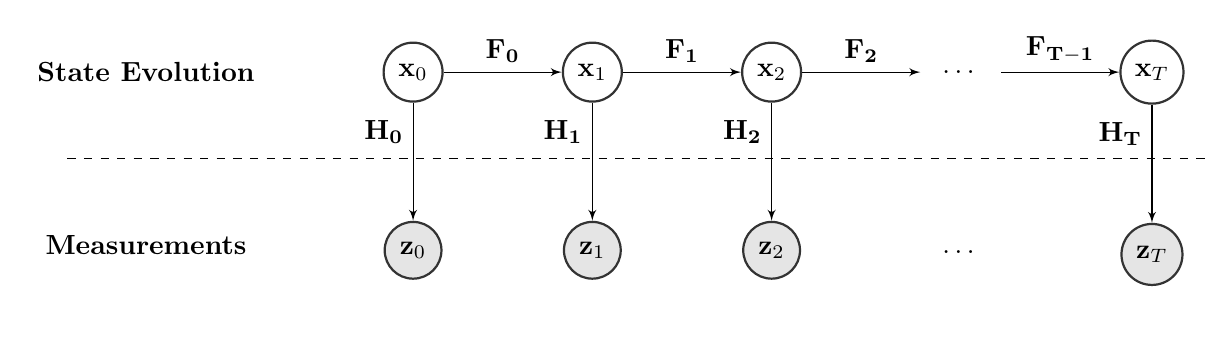
\begin{tikzpicture}[edge/.style = {->,> = latex'}]
	\node[box,draw=white!100] (Latent) {\textbf{State Evolution}};
	\node[main] (L1) [right=of Latent] {$\mathbf{x}_0$};
	\node[main] (L2) [right=of L1] {$\mathbf{x}_1$};
	\node[main] (L3) [right=of L2] {$\mathbf{x}_2$};
	\node[invis] (L4) [right=of L3] {};
	\node[main] (Lt) [right=of L4] {$\mathbf{x}_T$};
	\node[main,fill=black!10] (O1) [below=of L1] {$\mathbf{z}_0$};
	\node[main,fill=black!10] (O2) [below=of L2] {$\mathbf{z}_1$};
	\node[main,fill=black!10] (O3) [below=of L3] {$\mathbf{z}_2$};
	\node[invis] (04) [below=of L4] {};
	\node[main,fill=black!10] (Ot) [below=of Lt] {$\mathbf{z}_T$};
	\node[box,draw=white!100, below=of Latent, yshift=-7mm] (Observed) {\textbf{Measurements}};
	\path (L3) to node {\dots} (Lt);
	\draw[edge] (L1) to node[above] {$\mathbf{F_0}$} (L2);
	\draw[edge] (L2) to node[above] {$\mathbf{F_1}$} (L3);
	\draw[edge] (L3) to node[above] {$\mathbf{F_2}$} (L4);
	\draw[edge] (L4) to node[above] {$\mathbf{F_{T-1}}$} (Lt);
	\path (O3) to node {\dots} (Ot);
	\draw[edge] (L1) to node[near start, left] {$\mathbf{H_0}$} (O1);
	\draw[edge] (L2) to node[near start, left] {$\mathbf{H_1}$} (O2);
	\draw[edge] (L3) to node[near start, left] {$\mathbf{H_2}$} (O3);
	\draw[edge] (Lt) to node[near start, left] {$\mathbf{H_T}$} (Ot);
	
	% draw the dashed line
	\draw [dashed, shorten >=-1cm, shorten <=-1cm]
	($(Latent)!0.5!(Observed)$) coordinate (a) -- ($(Lt)!(a)!(Ot)$);
	\end{tikzpicture}
	\caption{\textbf{The KF as a Graphical Model} - In the vanilla KF $x^{(t)} \in \mathbb{R}^n$denotes the detection at time $t$, $z^{(t)} \in \mathbb{R}^m$ the measurement at $t$, $F^{(t)} \in \mathbb{R}^{n \times n}$ models the dynamics in the state space and $H^{(t)} \in \mathbb{R}^{m \times n}$ is the measurement function. The random variables are assumed to be gaussian distributed with $x^{(t+1)} \sim \mathcal{N}(Fx^{(t)}, Q^{(t)})$ and $z^{(t)} \sim \mathcal{N}(Hx^{(t)}, R^{(t)})$.}
	\label{graphical_model}
\end{figure}

\bigskip



\subsubsection{The State Space and State Evolution}
The state space holds all relevant information describing the current state of the system. The state $x^{(t)}$ holds information about the current 

$$\text{position } p^{(t)} = \left(p^{(t)}_x, p^{(t)}_y, p^{(t)}_z\right)\in \mathbb{R}^3 \text{ and  orientation } q^{(t)} = \left(q^{(t)}_w, q^{(t)}_x, q^{(t)}_y, q^{(t)}_z\right)\in \mathbb{R}^4,$$

 represented as a unit quaternion. Furthermore, the state holds information about the rate of change of $\smash{p^{(t)}}$ and $\smash{q^{(t)}}$. The exact form depends on the used motion models.\\
Assuming a constant velocity model for the position of the birds the state additionally estimates the current $$\text{velocity } v^{(t)} = \left( v^{(t)}_x, v^{(t)}_y, v^{(t)}_z\right) \in \mathbb{R}^3.$$ A brownian motion model for the quaternions is assumed, meaning that no additional information about the change of the quaternions is present in the state. This is justified by the complication that the function mapping from the state space to the measurement space is not known beforehand, the correction step of the KF might introduce large changes in the estimate for the quaternion. When using a for example a constant velocity model, these disruptions become even worse and impact the future frames more heavily than a brownian motion model. %TODO ist das verständlich?


With these assumptions the equations governing the state evolution are as follows:
\begin{eqnarray}
	p^{(t+1)} &=& p^{(t)} + v^{(t)} + \eta^{(t+1)}_{p} \label{pos_update} \qquad ~ \left( \eta_p \sim \mathcal{N}(0, \sigma_p \cdot I_3) \right)\\
	v^{(t+1)} &=& v^{(t)} + \eta^{(t+1)}_{v} \label{velocity_update} \qquad \qquad \quad \left( \eta_v \sim \mathcal{N}(0, \sigma_v \cdot I_3) \right)\\
	q^{(t+1)} &=& q^{(t)} + \eta^{(t+1)}_{q} \label{quat_update}  \qquad \qquad \quad \left( \eta_q \sim \mathcal{N}(0, \sigma_q \cdot I_4) \right)
\end{eqnarray}
, where $\sigma_p, \sigma_v$ and $\sigma_q$ are parameters determining the level of noise in the state evolution for the position, velocity and quaternion respectively. Putting this in a vectorized form gives the linear state transition function $F$ as a matrix for the KF:

\begin{equation}
	x^{(t+1)} = Fx^{(t)} = 
	\begin{pmatrix}
	1 & 0 & 0 & 1 & 0 & 0 & 0 & 0 & 0 & 0 \\
	0 & 1 & 0 & 0 & 1 & 0 & 0 & 0 & 0 & 0 \\
	0 & 0 & 1 & 0 & 0 & 1 & 0 & 0 & 0 & 0 \\
	0 & 0 & 0 & 1 & 0 & 0 & 0 & 0 & 0 & 0 \\
	0 & 0 & 0 & 0 & 1 & 0 & 0 & 0 & 0 & 0 \\
	0 & 0 & 0 & 0 & 0 & 1 & 0 & 0 & 0 & 0 \\
	0 & 0 & 0 & 0 & 0 & 0 & 1 & 0 & 0 & 0 \\
	0 & 0 & 0 & 0 & 0 & 0 & 0 & 1 & 0 & 0 \\
	0 & 0 & 0 & 0 & 0 & 0 & 0 & 0 & 1 & 0 \\
	0 & 0 & 0 & 0 & 0 & 0 & 0 & 0 & 0 & 1 \\
	\end{pmatrix}
	\begin{pmatrix}
	p^{(t)}_x \\
	p^{(t)}_y \\
	p^{(t)}_z \\
	v^{(t)}_x \\
	v^{(t)}_y \\
	v^{(t)}_z \\
	q^{(t)}_w \\
	q^{(t)}_x \\
	q^{(t)}_y \\
	q^{(t)}_z \\
	\end{pmatrix} + \eta 
\end{equation}, where $\smash{\eta \sim \mathcal{N}(0, diag(\sigma_p, \sigma_p, \sigma_p, \sigma_v, \sigma_v, \sigma_v, \sigma_q, \sigma_q, \sigma_q, \sigma_q))}$.

\subsubsection{The Measurement Space and Measurement Function}
\label{measurements}
The measurement function mapping from the state space to the measurement space is discussed next. In an ideal world, where no detections can be lost and the order of the detections is always the same, the relation of the measurement to the state is described by the following equation:

\begin{equation}
\tilde{H}(x^{(t)}) + \zeta= \begin{pmatrix}
\text{Rot}(q^{(t)})m_1 + p^{(t)} \\
\text{Rot}(q^{(t)})m_2 + p^{(t)} \\
\text{Rot}(q^{(t)})m_3 + p^{(t)} \\
\text{Rot}(q^{(t)})m_4 + p^{(t)} \\
\end{pmatrix} + \zeta= \tilde{z}^{(t)} \in \mathbb{R}^{12} \qquad \text{, where } \zeta \sim \mathcal{N}(0, \varrho \cdot I_{12})
\end{equation}

Since this measurement function is not linear and the quaternion has to be of unit norm the standard KF cannot be applied anymore. There are several variants of the EKF and UKF which deal with these issues. \cite{attitude_estimation} gives an overview the most common techniques. Interesting new approaches like \cite{manifolds} impose the manifold structure of the state space on the KF algorithm. %(In the case of estimating quaternions the state space is not the vector space $R^4$, but rather the unit sphere in $\mathbb{R}^4$, denoted by $S^3$)\\
I did not pursue any of the more elaborate approaches mentioned, yet, since the relation between the state and measurement space are more complicated, as explained next. Therefore the performance limiting factor is not the correct handling of the quaternions, but rather the detection-to-marker assignment.\\
Instead I chose to include the normalization of the quaternions in the function $\text{Rot}(.)$, mapping $q$ to a rotation matrix. %TODOThe definition of Rot() can be found in appendix \ref{quat_to_mat}.
 Note that this leaves the actual estimate for the quaternions unconstrained. Despite this, empirical results show that the the individual components of the quaternion estimates do not diverge further away from zero than 2.5. In future work investigating the performance gain of implementing a more suitable variant of the EKF or UKF would be interesting.

The actual measurement function needs to take the visibility and ordering of the detections into account. An algorithm to perform this detection-to-marker-assignment is discussed in section \ref{dtma}.
As stated in the problem formulation in section \ref{problem_def} detections are ordered in an arbitrary fashion, meaning that $z_{\lfloor i / 3 \rfloor}$ doesn't necessarily correspond to the $i\text{-th}$ marker. The correct function mapping from the system state to the measurements can then be expressed as follows:
\begin{equation}
H(x^{(t)}) + \zeta=
A^{(\pi^{t})} \begin{pmatrix}
\text{Rot}(q^{(t)})m_1 + p^{(t)} \\
\text{Rot}(q^{(t)})m_2 + p^{(t)} \\
\text{Rot}(q^{(t)})m_3 + p^{(t)} \\
\text{Rot}(q^{(t)})m_4 + p^{(t)} \\
\end{pmatrix} + \zeta
= z^{(t)} 
\end{equation}

, where $\smash{A^{(\pi^{t})}}$ is responsible for ordering and removing markers if they are not currently visible. 
Let $\smash{ \pi \in  \{1, \dots, K\}^1 \cup \dots \cup \{1, \dots, K\}^K}$ be a tuple dictating the ordering of the detections, where $\pi_i$ is the index of $i\text{-th}$ marker detected. In this definition I omit the possibility to classify all detections as false positives.\\
For a tuple $\pi$ of length $l$, $\smash{A^{(\pi)} \in \mathbb{R}^{l \cdot 3 \times d \cdot K}}$ can be defined as follows. The $3 \times 3$ block at block-index $i \in \{1, \dots l\}, j \in \{1, \dots, K\}$ is defined as
\begin{equation}
	A^{(\pi)}_{i,j} := \begin{cases}
							I_3, \quad \text{ if } \pi_i=j \\
							0_3, \quad \text{otherwise}
				  	       \end{cases}
\end{equation}.




%TODO: Why not use likelihood instead of distance?
\subsubsection{Detection to Marker Assignment}
\label{dtma}
The detection-to-marker-assignment is a crucial part of the proposed KF, as it estimates $\smash{\pi^{(t)}}$. Wrong estimates of $\smash{\pi^{(t)}}$ produce a false measurement function, which breaks down to whole concept of the KF. The position estimate is not strongly effected by such errors, since the rotation uses the position estimate as origin. The orientation estimate however suffers strongly from errors in estimating $\smash{\pi^{(t)}}$. Therefore the detection-to-marker assignment is designed to give the best possible estimate without regards of the runtime.\\

The estimation is done by energy minimization of a handcrafted energy $E$, which combines rotation and translation invariant information about the pattern of the object, as well as the prior knowledge of the rotation and translation as predicted by the KF. \\
Let there be $D$ point detections written as matrix of detections $X=(X_1, \dots, X_D)^T$. Let $m=(m_1, m_2, m_3, m_4)^T$ be the pattern of the object of interest.
Then any non-empty assignment $\pi$ of markers to detections can then be described by:
\begin{equation}
	\pi \in  \{1, \dots, 4\}^1 \cup \dots \cup \{1, \dots, 4 \}^D =: \Pi
\end{equation}, where $\pi_i = j$ means that the $i\text{-th}$ detection, $X_i$, is assigned the $j\text{-th}$ marker, $m_j$, of the pattern. Let M be the length of $\pi$. Allowing for $M<D$ means that detections can remain unassigned, which corresponds to classifying them as false positive detections, which frequently appear in practice.

The rotation and translation invariant part of the energy, $E_1(\pi)$ is defined as the mean squared error between the pairwise distances of the pattern  $m$ and the detections  $X$ brought into order by $\pi$:
\begin{equation}
	E_1(\pi) =  \frac{1}{\binom{M}{2}}\sum_{i =1}^M\sum_{j =i+1}^M \left( \left\| m_i - m_j\right\|_2 - \left\| X_{\pi_i} - X_{\pi_j}\right\|_2 \right)^2
\end{equation}

The second part of the energy, $E_2(\pi)$, makes use of the KF predictions  for position, $\hat{p}$,  and orientation, $\hat{q}$. Assuming that these predictions are good, which is not always the case in practice due to the simplified motion model, the rotated and translated pattern should be close to the detections ordered by $\pi$:

\begin{equation}
	E_2(\pi) = \frac{1}{M}\sum_{i =1}^M \left\| \text{Rot}(\hat{q})m_i + \hat{p}- X_{\pi_i}\right\|_2 
\end{equation}

Finally since $E_1(\pi)$ and $E_2(\pi) $ become small for small $M$, not assigning a detection to marker is punished with a fixed cost $c_{\text{nonAssignment}}$. The energy $E(\pi)$ is then composed of a weight sum of the three parts specified above:

\begin{equation}
	E(\pi) = \lambda_1 \cdot E_1(\pi) + \lambda_2 \cdot E_2(\pi) + (D-M) \cdot c_{\text{nonAssignment}}
\end{equation}

$E_1(\pi)$ is crucial in scenarios where the predictions are bad, $E_2(\pi)$ enforces temporal consistency and punishing non-assignments rewards longer $\pi$, which carry more information than short $\pi$.\\
Balancing the influences by choosing the parameters $\lambda_1, \lambda_2, c_{\text{nonAssignment}}$ was done in an empirical fashion with a very coarse grid search. %I determined $\lambda_1 = $, $\lambda_2 = $ and $c_{\text{nonAssignment}} = $%TODO put real values

The estimate 
$
	\hat{\pi} = \text{argmin}_{\pi \in \Pi} E(\pi)
$
is obtained by a simple exhaustive search over $\Pi$.



This exhaustive search heavily exploits the fact that $K=4$ and would not be practically possible for large $K$. In such cases an Iterative Closest Point(ICP) \cite{icp} algorithm could be used instead. Then it would be possible to only keep the matches with the highest certainty and discard the rest, since not all points are needed to estimated the rotation and translation and wrong matches could disrupt the KF. ICP is solving a problem very similar to what required in the detection-to-marker-assignment. Therefore it would be interesting to see how ICP compares to method described above, although I could not find information whether ICP works well with a small number of points, as local minima could potentially become a problem. \cite{icp_review} would be a good point to start searching for the right ICP variant for this specific problem.



\subsubsection{Some Heuristics}
\label{heuristics}
There are two notable heuristics I added to the KF approach.\\ Both are validated with experiments in section \ref{results_kalman_filter}.

\paragraph{False Positive Filtering} The detection-to-track-assignment is handled with the HA and a fixed cost for non-assignments. Having a fixed cost however is harmful, as the cost has to be high enough in order to allow for the erroneous prediction of the simplified motion model. Therefore if some or all actual detections are missing, false positive detections could be assigned to a track and if none ore only one true positive detection is assigned, it becomes hard to identify false positives, which leads to jumps in the predicted position and orientation and can cause to lose a track in the worst case. \\
To filter such false positives the non-assignment cost is scaled with velocity an object is currently moving, meaning that faster moving objects can still endure prediction errors of the motion model, while stationary objects get assigned less false positives.

\paragraph{Adaptive Noise} Similarly having a constant measurement noise scale $\varrho$
might be fitting for the regular KF setting, but as the measurement function is only estimated in this case, as described in the previous section, adapting the measurement noise to the certainty of the estimation of $\pi$ seems reasonable. Therefore the covariance matrix of the measurement noise is scaled by $E(\pi)$. This means that frames with a certain detection-to-marker-assignment will have a stronger influence on the state estimation.


\subsection{Deep Learning Approach}
\label{dl_approach}

The recent success of deep learning in many different areas also motivates to consider neural network for this task. The models described in the remainder of this section are SOT models and can be used in the MOT framework described in section \ref{approaches}.

\paragraph{Potential benefits}
I believe that the main benefits of a Deep Learning approach  compared to the KF approach are twofold: \\
First, a more complex motion model allows more accurate position predictions. While the relatively simple motion model of the KF might work well for predictions for the next time step, it especially breaks down when detections are missing for a few frames. A more complex motion model can accurately anticipate the next few time steps and therefore fill holes where detections are missing completely for multiple consecutive frames. This can potentially reduce the number of tracks being lost, which is important, since initializing new tracks can only be done in frames where the pattern can be determined with very high certainty, which occurs rarely.\\
Since there is some degree of non-determinism in the behavior of most objects, like in birds or pedestrians, predicting future positions is complicated. In order to tackle this problem, commonly multi-modal position predictions are used. Combining multi-modal predictions and long-term predictions is however far from trivial. \cite{multi_modal} present a possible solution for driver trajectory predictions in intersections. Whether such an approach is feasible for birds remains questionable, as the topology of the intersection strongly constrains possible trajectories.

Secondly, missed and false positive detections are a problem for the KF approach, as the simplified motion model does not carry over detailed information about the orientation to the detection-to-marker-assignment. A neural network can develop more complicated methods, which can draw more information from previous frames. The temporal information together with the position of the non-missing markers should be enough to reconstruct the positions of the missing markers, in order to estimate the rotation accurately.

\paragraph{Deep Learning specific Challanges} While Deep Learning looks like a promising method, designing an effective architecture is not trivial. In the following I list some of the problems that render the Deep Learning approach challenging:
\begin{itemize}
	\item Working on point clouds is problematic, as their input order should not be taken into account. Designing architectures which are invariant to the input order of detected points is tricky and described in section \ref{encoder}.
	\item Furthermore the network has to be capable of accepting a varying number inputs, as the amount of detections varies from frame to frame. This is also addressed in section \ref{encoder}
	\item Additionally the network has to perform well with every possible pattern, which is potentially of interest. In this case the neural network should work on all patterns used when recording the birds and on all patterns to be used in the future, as frequent retraining is tedious.
	\item Analytically estimating rotation and translation between two point clouds can be done with ICP or \cite{umeyama}, if the correspondences are known. However, this task alone is already non-trivial for neural networks, as described in section section \ref{rotation_representation}.\\
	Alternatively one could avoid estimating rotations directly, by just regressing the marker positions directly and calculating the rotations and translation in a post-processing step with \cite{umeyama}. I haven't followed this approach yet.
	\item Where to insert the temporal information as well as how to incorporate the pattern of the tracked object are both not obvious. The overall proposed architecture will be discussed next.

\end{itemize}


\subsubsection{Proposed Architecture}
\label{architecture}
The general architecture consist of an encoder neural network which maps the detected point cloud and the pattern of the tracked object to a more suitable, high dimensional representation, which is fed into the LSTM network. Note that since the pattern is not changing while tracking, it does not need to be fed into the network every step. For example It would be possible to initialize the hidden state from the pattern. The final hidden state of the LSTM is then mapped to position and orientation estimates, as well as, predicted position and orientation change for the next frame.
Figure \ref{NN_architecture}
shows the architecture on a high level. The exact form of the encoder is described in section \ref{encoder} and is a less obvious choice, while using a LSTM to transfer temporal information and an MLP network as regressor is quite natural.\\
Yet another approach would be to split up the task into two subtasks. The first would be classifying the detections into which marker they correspond to or whether they are false positive detections. This would correspond to a detection-to-marker-assignment. Then one could bring the detections into order and remove the false positives. A second network would then operate on the ordered detections, which makes the task of the second network significantly easier. I believe however, that imposing this structure onto the neural network is inferior opposed to leaving the neural network all freedom. Therefore I did not pursue this method.

\begin{figure}[!htbp]
	\begin{center}
		\subfigure[General Architecture]{%
			\label{NN_architecture}
			\includegraphics[scale=0.2]{img/NN_architecture.png}
		}
		\subfigure[Regressor Architecture]{%
			\label{NN_regressor}
			\includegraphics[scale=0.17]{img/NN_regressor.png}
		}
	\end{center}
	\caption{The neural network gets the detections at each frame, $X_t$ and pattern$m$ as input and predicts the current position $\hat{p}_t$ and rotation $\hat{r_t}$. Additionally the change in position and orientation to the next frame, $\smash{\widehat{\delta p}_t}$ and $\smash{\widehat{\delta r}_t}$, are predicted. These can be used for predicting the state in the next frame and for the detection-to-track-assignment. (a) The LSTM cell has 600 hidden units in all experiments. (b) The input is the hidden state of the LSTM at time step $t$. The numbers indicate the used number of hidden units. The dropout rate was set to 0.25. Using an additional fully connected layer in the regressor did not make a real difference in performance.}
\end{figure}

\subsubsection{Encoder Architecture}
\label{encoder}
As the detections come in an arbitrary ordering the encoder network has to be invariant to permutations of the inputs, i.e. it has operate on point clouds. This exact challenge is discussed in \cite{PointNet}. The authors designed an effective and efficient deep learning architecture, which works on point clouds and therefore is permutation invariant. Their approach is on par with other approaches, like Voluminetric CNNs \cite{VCNN} and Multi-view CNNs \cite{MVCNN}, while being computationally much more efficient. Voxelization and rendering images from multiple views does not seem to make sense for 4 points anyways.\\
Another alternative discussed in the paper is treating the detections as a sequential signal and training a Recurrent Neural Network (RNN) on randomly permuted sequences, hoping that the network will become permutation invariant. They found, that this approach is worse than their proposed architecture. The paper "Order Matters" \cite{orderMatters} gives various examples where input (and output) order in set2seq (seq2set) problems made a significant difference on performance, implicating that RNNs in general cannot be trained to become order invariant. However they suggest that for short  sequences (in their experiment they used a of length 5) the RNN seemed to less affected by the ordering.\\
Both papers did not mention MLPs, as they cannot deal with variable sequence length. In this problem however one can pad  the assigned detections with zeros and introduce an indicator variable masking the padded points. Then there are always 4 assigned detections as input and an MLP can be applied. \\
The architectures are depicted in figure \ref{encoder_architecture}.
In section \ref{results_dl} I will compare the performance of a PointNet-sytle encoder, a LSTM encoder and a MLP encoder.

%TODO can confirm order matters in MLP, lost dets to the end

\begin{figure}[!htbp]
	\begin{center}
		\subfigure[MLP Encoder]{%
			\label{NN_mlp_encoder}
			\includegraphics[scale=0.18]{img/NN_mlp_encoder.png}
		}
		\subfigure[LSTM Encoder]{%
			\label{NN_lstm_encoder}
			\includegraphics[scale=0.19]{img/NN_lstm_encoder.png}
		} 
		\subfigure[PointNet-style Enocder]{%
			\label{NN_pointnet_encoder}
			\includegraphics[scale=0.22]{img/NN_pointnet_encoder.png}
		}
	\end{center}
	\caption{For all architectures the detections are padded with zeros and a variable indicating the padded entries, such that $X_t \in \mathbb{R}^{6\times4}$. For (a) and (b) the detections are shuffled such that the network learns to become permutation invariant. For (a) moving the passed zeros to the back was greatly beneficial. (c) is a similar architecture to the PointNet \cite{PointNet} architecture, except that no matrix transform is applied as translation rotation is of interest. Therefore the detection order has no effect on the network. The features after the first pooling operation hold information about the whole point cloud. These are concatenated with the local features after the second 1d convolution in order to combine both local and global information. Whether sharing weights makes sense has to be tested, as the only one part has to deal with noise. Furthermore the pattern-network-part always gets the same pattern meaning that a simple MLP network would be sufficient.}
	\label{encoder_architecture}
\end{figure}

\subsubsection{Representing Rotations}
\label{rotation_representation}
Choosing a suited rotation representation method for neural networks is essential. Most common representations as Euler angles and quaternions suffer from certain discontinuities, as described in \cite{rotation_representation}. The paper proposes an alternative continuous 6-dimensional representation for rotations in 3-dimensional space, which alleviates the problems of discontinuous representations.  My empirical results support these findings, see section \ref{results_dl}. The authors argue that instead of directly regressing the rotation matrix, which would not suffer from discontinuities, and then applying a Gram-Schmidt process to orthogonalize it, it is possible to regress 6 parameters, which can be mapped to a rotation matrix with the following simple mapping:
{
\begin{eqnarray*}
	\text{Rot}\begin{pmatrix}
		| & | \\
		a_1 & a_2 \\
		| & | 
	\end{pmatrix} &:=& \begin{pmatrix}
		| & | & |\\
		b_1 & b_2 & b_3\\
		| & | & |
	\end{pmatrix}
	\qquad \text{, where} \\
b_1 &:=& \frac{a_1}{\| a_1\|_2} \\
b_2 &:=& \frac{a_2 - \langle b_1, a_2\rangle b_1}{\| a_2 - \langle b_1, a_2\rangle b_1\|_2} \\
b_3 &:=& b_1 \times b_2
\end{eqnarray*}
}


\section{Results}
\label{results}

\subsection{Generating Data}
As there is no labeled data of the birds available, I had to generate data myself, in order to evaluate the performance of the models quantitatively. However generating realistic bird behavior from scratch is difficult, I took two different approaches. First I generated random 3d trajectories and orientation trajectories by composing functions from multiple simple functions. The generate behavior is far from actual bird behavior, however I tried to come up with a wide variety of data in order to test the generality of the models. I denote this data set by "artificial" data. Additionally I generated data based on the KF predictions in the real detections. I smoothened the predictions and only used parts without obvious errors, like discontinuities or extreme motion or rotation. This data is denoted by "birdlike".\\
Equally important as the generate underlying behavior is the simulation of the detections and introducing realistic measurement errors. I came up with two random processes to simulate the presence of false positive detections as well as missed detections. These random processes are solely inspired by observing the real detections and the following two observations: First missing detections do not occur uniform at random. It seems that rather some markers go missing for multiple frames at a time, before producing reliable detections again. This could be explained by bird covering a marker with a feather for some time. Second false positive detections also do not appear uniformly at random. There seem to be some points in the room which sometimes reflect the infrared light for certain periods.\\
Using these stochastic processes allows to specify the amount of noise present.

\subsection{Experimental Results}
\subsubsection{Evaluating the Kalman Filter Approach}
\label{results_kalman_filter}

Figure \ref{KF_mot_metrics} shows the MOTA and Pose-MOTP metrics on a birdlike dataset with 10 birds present. Therefore, this experiment is a bit biased, as the result of the KF were used to obtain the underlying trajectories. However the noise levels were simulated with the two stochastic processes, as described in the previous section, meaning that this experiment is still fit to investigate the noise resistance of the different KF versions. The videos found in \href{https://github.com/SimonGiebenhain/tracking}{GitHub} also show the MOT results on the real detections. The results seem to be of high quality, indicating that even the most simple motion model combined with the HA is sufficient to master the detection-to-track-assignment. In the following I explain the effects of the three investigated additions to the most simple KF version.\\ 

\textbf{Proposed detection-to-marker-assignment}  \space \space\space  The only version using this detection-to-marker-assignment, as described in section \ref{dtma}, are \emph{noAdaptiveNoise} and \emph{all}. It is clear to see that the Pose-MOTP error is drastically lower when using this method instead of a simple HA on distances of the detections to predicted marker locations. When comparing the Pose-MOTP of \emph{simplePatternMatching} and \emph{all}, which only differ in the detection-to-marker-assignment, one observes that the simple detection-to-track-assignment never really manages to predict the correct pose, even in low noise levels. The effect on the MOTA is less obvious. \\
\textbf{False positive filtering}\space \space\space This heuristic, as explained in section \ref{heuristics}, is used in all versions except in \emph{all}, and is the only difference between \emph{all} and \emph{onlyFPFiltering}. Clearly both the Pose-MOTP and especially the MOTA are strongly positively influenced by this heuristic.\\
\textbf{Adaptive Noise} \space \space\space The effect of this heuristic, as described in section \ref{heuristics}, can be seen when comparing the version \emph{noAdaptiveNoise} and \emph{all}, which only differ in the use of adaptive noise. Both the Pose-MOTP but especially the MOTA are positively influenced by this method.

\begin{figure}[!htbp]
	\begin{center}
		\subfigure[Pose-MOTP]{%
			\label{NN_mlp_encoder}
			\includegraphics[scale=0.4]{img/Pose-MOTP.png}
		}
		\subfigure[MOTA]{%
			\label{NN_lstm_encoder}
			\includegraphics[scale=0.4]{img/MOTA.png}
		} 

	\end{center}
	\caption{\textbf{KF performance on different noise levels} - These results compare the MOTA and Pose-MOTP for different noise levels and different versions of the KF. \emph{none} refers to the most simple Kalman Filter with no additions and the HA for the detection-to-marker-assignment. \emph{onlyFPFiltering} is the same as \emph{none} with the addition of false positive filtering as described in section \ref{heuristics}. \emph{simplePatternMatching} has both false positive filtering and adaptive noise, as describe in section \ref{heuristics}, but also the same simple detection-to-marker-assignment as \emph{none}. \emph{noAdaptiveNoise} uses the detection-to-marker-assignment described in section \ref{dtma}, false positive filtering but no adaptive noise. \emph{all} uses all the additions. Note the y-axis range for figure (b).}
	\label{KF_mot_metrics}
\end{figure}

\subsubsection{Evaluating the Deep Learning Approach}
\label{results_dl}

\paragraph{Training Procedure}
In order to ease the training of the neural network, a simplified task is considered. The training data consists of 50.000 sequences of 100 frames each. The test dataset hold 5.000 sequences of length 100. However each sequence is scaled an shifted such that the mean of each sequence is 0 and the standard deviation over the norms of each position in each sequence is 1. This way the training data densely covers the vicinity of the origin and makes training a lot easier. This simplification has the drawback that the neural network cannot be easily applied to a long sequence anchored at an arbitrary position in the room.\\
Furthermore the neural network is only evaluated as a SOT. Therefore predicting $\smash{\widehat{\delta p}}$ and $\smash{\widehat{\delta r}}$ is skipped. \\
The networks are trained for 100 epochs with a batch size of 64. The Adam optimizer with an initial learning rate of 0.001 and a momentum of 0.9 is used. The learning rate is reduced with a factor of 0.5 upon hitting a plateau. Here a patience of 3 and cooldown of 10 epochs is used. Furthermore weight decay with a weight decay of 0.0002 is applied. \\
The resulting performance can be found in table \ref{pose_error_results}.

\paragraph{Comparing Encoder Architectures}
The results in table \ref{pose_error_results} clearly show that the MLP encoder works best in all settings. It is interesting to note that the LSTM encoder works quite well in a noise free setting, but is heavily affected by increasing noise levels. Despite the promising results of \cite{PointNet} the PointNet encoder did not work well. It has to be noted that the training pose error was comparable to the other models. However I was not able to overcome this severe overfitting, despite introducing more dropout, a higher weight decay and fewer parameters. I cannot explain this behavior and further investigation of this issue is necessary.

\paragraph{Comparing Rotation Representation}
The results in table \ref{pose_error_results} suggest that representing rotations as unit quaternions introduces issues in neural networks and matches with the findings of \cite{rotation_representation}. It is interesting to see that the pose error does not drastically increase with increasing noise. This suggests that not the noise is the main problem but rather the rotation representation itself.\\


\begin{table}[h!]
	\centering
	\begin{tabular}{|l|l |c| c| c|} 
		\hline
		model type & model + rotation representation & no noise & medium noise & high noise \\ \hline
		\hline
		NN & MLPencoder + 6d & \textbf{0.032} & \textbf{0.042} & \textbf{0.077} \\ \hline
		NN & MLPencoder + quat & 0.112 & 0.108 & 0.150 \\ \hline
		NN & LSTMencoder + 6d & 0.057 & 0.164 & 0.243 \\ \hline
		NN & PointNetEncoder + 6d & 0.468 & 0.710 & 0.696 \\ \hline \hline
		KF & proposedKF + quat       & \textbf{0.008} & \textbf{0.011} & \textbf{0.031} \\
		\hline
	\end{tabular}\\
	\bigskip
	\caption{\textbf{Comparing pose error of different models on artificial data} - The experiments presented here were conducted on artificial data of a single object. The used metric is the pose error, similar two the Pose-MOTP defined in section \ref{problem_def}, but in a SOT setting. All models were evaluated on different noise levels. The evaluated neural network models only differ in the encoder architecture, as discussed in \ref{encoder_architecture} and the best neural network performing model was also evaluated with internally representing rotations as quaternions, in order to show the dominance of the 6d rotation representation explained in \ref{rotation_representation}.  The proposed KF was evaluated on the same data. }
	\label{pose_error_results}
\end{table}



\subsection{Comparing both approaches}
\label{comparison}
The results of the MLP encoder network and the KF approach in both tables \ref{pose_error_results} and \ref{table_KF_vs_NN} suggest that the neural network is inferior to he KF approach, despite the fact that the data was generate in a form, which rendered training the neural network  easier, as describe in section \ref{results_dl}. However, the neural network seems to be less influenced by increasing noise levels. The neural network is already inaccurate in a noise free setting. Thus there might be some flaws in the architecture, as it should be possible to achiever near perfect results in a noise free setting. Once these issues have been resolved, the higher resistance to noise could make the neural network perform better than the KF. \\
The KF also performed better on the birdlike data, as the trajectories are simpler than in the artificial data. This is due to the simplified motion model of the KF. \\
Another advantage of the KF is its generality. It makes no assumption about the behavior or the patterns of the objects. Therefore only a few parameters might have to be changed in order to apply the model to a completely new setting. Although I have not investigated the generality of the neural network by evaluating it on different kinds of data than training it on, for certain changes to the setup a complete retraining might be necessary. \\
One drawback of the KF is the assumption that $K$ is small, as the detection-to-track-assignment consumes exponential time in $K$.

\begin{table}[h!]
	\centering
	\begin{tabular}{|l |c| c| c|} 
		\hline
		model &  medium noise & high noise \\ \hline
		\hline
		proposedKF &  \textbf{0.0025} & \textbf{0.0055} \\ \hline
		MLPencoder + 6d &  0.0348 & 0.045 \\ 
		\hline
	\end{tabular}\\
	\bigskip
	\caption{\textbf{Comparing pose error on birdlike data} -  The experiments followed the same setup as in table \ref{pose_error_results}. However the numbers cannot be directly compared, as the data had different scale due to the normalization procedure.}
	\label{table_KF_vs_NN}
\end{table}
\section{Future Work}
\label{future_work}

The KF already produced decent results, despite not treating the quaternions correctly, only being an EKF and using a very simple motion model. In future I will investigate slightly more sophisticated motion models and use a version of the EKF which treats the quaternions appropriately. Another interesting line of research is estimating the parameters of the KF, as they have to hand tuned as of now. Whether one of the common approaches, like Expectation Maximization for parameter estimation, is applicable to this setting remains to be seen. Not knowing and only estimating the measurement function might introduce problems. \\
The deep learning approach is showing promising results in terms of noise resistance, but still makes mistakes in a noise free setting. This suggests that the architecture is not optimal yet. In the following I list some ideas how to improve the neural network. The experiments showed that the rotation representation can be the limiting factor. Therefore directly regressing the marker positions is an alternative approach which bypasses representing rotations. As regressing points is successfully done in practice, e.g. human joints or bounding boxes, this approach seems promising. \\
Furthermore, the neural networks are not capable of tracking for long, as they are only trained on short sequences implying that the object cannot leave far from the origin. Resolving this issue will be of future work. \\
Another issue is making the encoder permutation invariant. Training a MLP to become permutation invariant seems wasteful. However the PointNet architecture overfit severely. In future I will investigate this issue. However only working with 4 points could explain the bad performance, as PointNet normally is applied to dense meshes.\\
The fact that all detections of a single bird sometimes go missing for multiple consecutive frames, encourages further investigation of the neural network approach, since a more sophisticated motion model can potentially fill these holes and prevent the track from getting lost. \\
Yet another possibility is to combine both approaches, by training a neural network to perform the detection-to-track-assignment in the KF approach.


%The solid performance of the KF approach shows that a simple position prediction method, like a constant velocity model, is enough in most cases to maintain the tracks over time and inhibit ID-switches. Since the position of birds does not change drastically within a single time step, the detection to track assignment, which is the most critical step in MOT, is relatively easy. However the exact detection to marker assignment is harder already. However an exact detection to marker assignment is not strictly necessary, since error introduced by such are quite small. \\
%There are however two major difficulties that remain:
%First, orientation estimation is especially challenging because small mistakes in the detection to marker assignment or an undetected FP can completely disrupt the estimation. This problem could be tackled with better heuristics Since coming up with viable heuristics can be very tedious, a Neural Network could be trained to handle the detection to marker assignment. Such an approach will be subject of future research.\\
%Secondly long term predictions are are required to fill gaps in cases with no or very few detections for multiple consecutive frames. As \cite{tracking_the_trackers} found, most MOT algorithms increase the FN rate, instead of decreasing it by filling in gaps. This leads to the conclusion that \emph{trajectory prediction literature} seems more promising than \emph{MOT literature} to tackle the problem at hand. Since even the simple constant velocity motion model of the EKF was sufficient to produce good position estimation and inhibit any ID-switches, it seems reasonable to disregard the tracking of multiple objects, focus on good trajectory prediction and obtain MOT by the HA and simple heuristics to manage the birth and death of tracks.

\section{Conclusion}

In this work, a new kind of MOT was formulated. Experiments showed that the detection-to-track-assignments, which is commonly the most challenging part of MOT, is simple. Therefore, the difficulty lies in the precise tracking of position and orientation for single objects, which are then combined to MOT with a distance based HA for the detection-to-track-assignment and a few simple heuristics. Both introduced model are SOT for this framework. A simple EKF with a few additions to handle specific difficulties quantitatively achieves good results on generate data. A qualitative observation of the MOT results on the real data confirms the good results. The neural network based SOT introduced here still needs improvement, but already shows promising noise resistance. Several improvement ideas for both models are given.

\bibliographystyle{apalike}  
\bibliography{references}

%\begin{appendices}
%
%\section{Quaternions}
%\subsection{From Quaternions to Rotation Matrices}
%\label{quat_to_mat}
%% TODO


%\end{appendices}


\end{document}
